\documentclass[xcolor=dvipsnames, handout]{beamer}
\usetheme{presentation}
\usepackage[round]{natbib}
\usepackage{bibentry}
\definecolor{citecolor}{gray}{0.6}
\let\oldcitep\citep
\renewcommand{\citep}[1]{{\color{citecolor}\tiny\oldcitep{#1}}}
\nobibliography*
%\usepackage[cjk]{kotex}
%\usepackage{listings}
\usepackage{tikz}
\usetikzlibrary{arrows.meta}
\tikzset{
    invisible/.style={opacity=0},
    visible on/.style={alt={#1{}{invisible}}},
    alt/.code args={<#1>#2#3}{%
      \alt<#1>{\pgfkeysalso{#2}}{\pgfkeysalso{#3}} % \pgfkeysalso doesn't change the path
    },
}
% ----------------------------- Title & Author ------------------------------ %
\title{Causal Inference with Ordinal Outcomes}
\subtitle{Density Estimation Based Approach}
\author{Chanhyuk Park}
\institute{Washington University in St. Louis}
\date{}

\begin{document}
   \frame{\titlepage}
\begin{frame}{Motivation: The Discretization Problem}
    \begin{itemize}
        \item Experiments to identify causal effects of treatments
        \pause 
        \item Outcomes are usually believed to be continuous in unidimensional space
            \begin{itemize}
                \item Approval ratings \citep{Canes-Wrone2002a, Kriner2009a}
                \item Policy preferences \citep{Scheve2001r, Mayda2005a, Wu2022a}
            \end{itemize}
        \pause
        \item The Problem - How we measure it
    \end{itemize}

    \vspace{0.5cm}

    \centering
    % The Latent Axis Line and its label appear on Step 2 and persist.
    \only<3->{
        \begin{tikzpicture}[font=\sffamily, thick]
            % --- Main Axis (Always Black and No Arrow) ---
            \begin{scope} 
                % Removed '->' to get rid of the arrow
                \draw[very thick, black] (0,0) -- (10,0); 
                \foreach \x in {0, 10} \draw (\x, 0.2) -- (\x, -0.2);
                % Axis Label
                \node[above, yshift=5pt] at (5, 0) {\textbf{The True Outcome}};
            \end{scope}

            % --- Step 3: First Arbitrary Bracketing ---
            \only<4>{
                \begin{scope} 
                    % Partition A Cut-Points
                    \foreach \x in {2, 4.5, 6, 8.5} \draw (\x, 0.2) -- (\x, -0.2);

                    % Brackets (Hanging Arches)
                    \draw (0,-0.2) to [out=-90, in=150] (1, -1.2);
                    \draw (2,-0.2) to [out=-90, in=30] (1, -1.2);
                    
                    \draw (2,-0.2) to [out=-90, in=150] (3.25, -1.2);
                    \draw (4.5,-0.2) to [out=-90, in=30] (3.25, -1.2);

                    \draw (4.5,-0.2) to [out=-90, in=150] (5.25, -1.2);
                    \draw (6,-0.2) to [out=-90, in=30] (5.25, -1.2);
                    
                    \draw (6,-0.2) to [out=-90, in=150] (7.25, -1.2);
                    \draw (8.5,-0.2) to [out=-90, in=30] (7.25, -1.2);
                    
                    \draw (8.5,-0.2) to [out=-90, in=150] (9.25, -1.2);
                    \draw (10,-0.2) to [out=-90, in=30] (9.25, -1.2);

                    % Bottom Labels
                    \node at (1, -1.5) {\scriptsize\itshape Strongly Agree};
                    \node at (3.25, -1.5) {\scriptsize\itshape Agree};
                    \node at (5.25, -1.5) {\scriptsize\itshape Neither};
                    \node at (7.25, -1.5) {\scriptsize\itshape Disagree};
                    \node at (9.25, -1.5) {\scriptsize\itshape Strongly Disagree};
                \end{scope}
            }

            % --- Step 4: Second Arbitrary Bracketing ---
            \only<5>{
                \begin{scope} 
                    % Partition B Cut-Points
                    \foreach \x in {3, 4, 5, 9} \draw (\x, 0.2) -- (\x, -0.2);

                    % Brackets
                    \draw (0,-0.2) to [out=-90, in=150] (1.5, -1.2);
                    \draw (3,-0.2) to [out=-90, in=30] (1.5, -1.2);
                    
                    \draw (3,-0.2) to [out=-90, in=150] (3.5, -1.2);
                    \draw (4,-0.2) to [out=-90, in=30] (3.5, -1.2);

                    \draw (4,-0.2) to [out=-90, in=150] (4.5, -1.2);
                    \draw (5,-0.2) to [out=-90, in=30] (4.5, -1.2);
                    
                    \draw (5,-0.2) to [out=-90, in=150] (7, -1.2);
                    \draw (9,-0.2) to [out=-90, in=30] (7, -1.2);
                    
                    \draw (9,-0.2) to [out=-90, in=150] (9.5, -1.2);
                    \draw (10,-0.2) to [out=-90, in=30] (9.5, -1.2);

                    % Bottom Labels
                    \node at (1.5, -1.5) {\scriptsize\itshape Strongly Agree};
                    \node at (3.5, -1.5) {\scriptsize\itshape Agree};
                    \node at (4.5, -1.5) {\scriptsize\itshape Neither};
                    \node at (7, -1.5) {\scriptsize\itshape Disagree};
                    \node at (9.5, -1.5) {\scriptsize\itshape Strongly Disagree};
                \end{scope}
            }
        \end{tikzpicture}
    }
\end{frame}

\begin{frame}{The Goal}
    \begin{itemize}
        \item<1-> \textit{\color<2->{purple}Identification} \\
            \only<2->{
                Naive causal identification with these "index" may fail \\
                \vspace{0.2cm}
                $\implies$ \textcolor{purple}{Normalized Latent Treatment Effect}
            }
            \vspace{0.5cm}
        \item<1-> \textit{\color<3->{orange}Estimation} \\
            \only<3->{
                Standard parametric regression is rigid \\
                \vspace{0.2cm}
                $\implies$ \textcolor{orange}{Flexible, density estimation} based estimators
            }
    \end{itemize}
\end{frame}

\begin{frame}{Why Naive Identification Fails}
    \vspace{0.5cm}
    \centering
        \begin{tikzpicture}[font=\sffamily, thick]
            % --- Main Axis (Always Black and No Arrow) ---
            \begin{scope} 
                % Removed '->' to get rid of the arrow
                \draw[very thick, black] (0,0) -- (10,0); 
                \foreach \x in {0, 10} \draw (\x, 0.1) -- (\x, -0.1);
                \foreach \x in {2, 4.5, 6, 8.5} \draw (\x, 0.1) -- (\x, -0.1);
                % Axis Label
                \node[above, yshift=5pt] at (5, 0.5) {\textbf{The True Outcome ($\boldsymbol{Y^{\ast}}$)}};
                % Top Labels
                \node at (0, 0.3) {\scriptsize\itshape 0};
                \node at (10, 0.3) {\scriptsize\itshape 10};
            \end{scope}

            % --- DGP ---
            % \only<2->{
            %     \begin{scope} 
            %         % Partition A Cut-Points
            %
            %         % Brackets (Hanging Arches)
            %         \draw (0,-0.2) to [out=-90, in=150] (1, -1.2);
            %         \draw (2,-0.2) to [out=-90, in=30] (1, -1.2);
            %
            %         \draw (2,-0.2) to [out=-90, in=150] (3.25, -1.2);
            %         \draw (4.5,-0.2) to [out=-90, in=30] (3.25, -1.2);
            %
            %         \draw (4.5,-0.2) to [out=-90, in=150] (5.25, -1.2);
            %         \draw (6,-0.2) to [out=-90, in=30] (5.25, -1.2);
            %
            %         \draw (6,-0.2) to [out=-90, in=150] (7.25, -1.2);
            %         \draw (8.5,-0.2) to [out=-90, in=30] (7.25, -1.2);
            %
            %         \draw (8.5,-0.2) to [out=-90, in=150] (9.25, -1.2);
            %         \draw (10,-0.2) to [out=-90, in=30] (9.25, -1.2);
            %
            %         % Bottom Labels
            %         \node at (1, -1.5) {\scriptsize\itshape Strongly Agree};
            %         \node at (3.25, -1.5) {\scriptsize\itshape Agree};
            %         \node at (5.25, -1.5) {\scriptsize\itshape Neither};
            %         \node at (7.25, -1.5) {\scriptsize\itshape Disagree};
            %         \node at (9.25, -1.5) {\scriptsize\itshape Strongly Disagree};
            %
            %
            %     \end{scope}
            % }

            % --- Introduce Reporting Function ---
            \only<3->{
                \begin{scope}[purple]
                    % Partition A Cut-Points

                    % Brackets (Hanging Arches)
                    \draw (0,-0.2) to [out=-90, in=150] (1, -1.2);
                    \draw (2,-0.2) to [out=-90, in=30] (1, -1.2);
                    
                    \draw (2,-0.2) to [out=-90, in=150] (3.25, -1.2);
                    \draw (4.5,-0.2) to [out=-90, in=30] (3.25, -1.2);

                    \draw (4.5,-0.2) to [out=-90, in=150] (5.25, -1.2);
                    \draw (6,-0.2) to [out=-90, in=30] (5.25, -1.2);
                    
                    \draw (6,-0.2) to [out=-90, in=150] (7.25, -1.2);
                    \draw (8.5,-0.2) to [out=-90, in=30] (7.25, -1.2);
                    
                    \draw (8.5,-0.2) to [out=-90, in=150] (9.25, -1.2);
                    \draw (10,-0.2) to [out=-90, in=30] (9.25, -1.2);

                    % Bottom Labels
                    \node at (1, -1.5) {\scriptsize\itshape Strongly Agree};
                    \node at (3.25, -1.5) {\scriptsize\itshape Agree};
                    \node at (5.25, -1.5) {\scriptsize\itshape Neither};
                    \node at (7.25, -1.5) {\scriptsize\itshape Disagree};
                    \node at (9.25, -1.5) {\scriptsize\itshape Strongly Disagree};
                \end{scope}
            }
            % --- Common Index / Cardinalization ---
            \only<4->{
                \begin{scope}[blue]
                    % Arrows to top
                    \draw[->] (1,-1) to (1, -0.2);
                    \draw[->] (3.25,-1) to (2, -0.2);
                    \draw[->] (5.25,-1) to (3, -0.2);
                    \draw[->] (7.25,-1) to (4, -0.2);
                    \draw[->] (9.25,-1) to (5, -0.2);

                    % Top Labels
                    \node at (1, 0.4) {\footnotesize\itshape 1};
                    \node at (2, 0.4) {\footnotesize\itshape 2};
                    \node at (3, 0.4) {\footnotesize\itshape 3};
                    \node at (4, 0.4) {\footnotesize\itshape 4};
                    \node at (5, 0.4) {\footnotesize\itshape 5};

                    % Bottom Labels
                    \node at (1, -1.5) {\scriptsize\itshape Strongly Agree};
                    \node at (3.25, -1.5) {\scriptsize\itshape Agree};
                    \node at (5.25, -1.5) {\scriptsize\itshape Neither};
                    \node at (7.25, -1.5) {\scriptsize\itshape Disagree};
                    \node at (9.25, -1.5) {\scriptsize\itshape Strongly Disagree};
                \end{scope}
            }
        \end{tikzpicture}
    \vspace{0.5cm}
    \pause
    \begin{itemize}[<+->]
        \item The treatment effect we want: $\E{Y^{\ast}(1)} - \E{Y^{\ast}(0)}$
        \item \textit{\color{purple} Unknown Reporting Function $g$}
        \item \textit{\color{blue} Arbitrary index $f$}
        \item The treatment effect we get: $\E{{\color{blue}f}({\color{purple}{g}}(Y^{\ast}(1)))} - \E{{\color{blue}f}({\color{purple}{g}}(Y^{\ast}(0)))}$
    \end{itemize}
\end{frame}

\begin{frame}{Normalization}
    \begin{itemize}[<+->]
        \item Unobserved $Y^{\ast}$ and Unknown $g$ \\ 
            $\implies$ identify LTE up to scale \\ 
            $\implies$ treatment effect $\tau^{\ast}$ cannot be distinguished form $C\tau^{\ast}$
            \vspace{0.4cm}
        \item Normalization to cancel out $C$
        \begin{itemize}
            \item {\color<6->{blue} Scale to fix $\sigma_{\varepsilon_{i}} = 1$} \\
                \only<6->{\color{blue}
                    \vspace{0.2cm}
                    $\implies \frac{\tau^{\ast}}{\sigma_{\varepsilon_{i}}}$ is identified
                    \vspace{0.2cm}
                }
            \item<4-5> If there are multiple treatments, fixing $\tau_{a} = 1$
            \item<5-5> Pure probability scale
        \end{itemize}   
    \end{itemize}
\end{frame}

\begin{frame}{How Can We Estimate?}
    \begin{itemize}
        \item Ordered Probit, Ordered Logit, and most IRT models \\
            $\implies$ Assume that $\varepsilon_i$ follows specific distributions \pause
            \vspace{0.3cm}
        \item Distributional Assumptions can be violated
            \begin{itemize}
                \item Pure misspecification
                \item Unobserved confounder
            \end{itemize} \pause
            \vspace{0.2cm}
        \item Become \textit{inconsistent} \pause
            \vspace{0.3cm}
        \item \textcolor{blue}{Two Flexible Estimators} without rigid Distributional Assumptions
    \end{itemize}
\end{frame}

\begin{frame}{Alternative: Estimate the Distribution}
    \begin{itemize}
        \item<1-> Nonparametric method: \textcolor{purple}{Kernel Density Estimation}
            \only<2->{
                \begin{itemize}
                    \item Smooth each observation using a kernel (usually Gaussian)
                        $$
                        \hat f(x)
                        = \frac{1}{n h} \sum_{i=1}^n K\!\left( \frac{x - X_i}{h} \right)
                        $$ 
                \end{itemize}
            }
            \vspace{0.6cm}
        \item<1-> Parametric Generative Model: \textcolor{orange}{Normalizing Flows}
            \only<3->{
                \begin{itemize}
                    \item Use the change-of-variable formula
                        $$
                        f_\theta(h)
                        = f_Z\bigl(T_\theta^{-1}(h)\bigr)
                        \left|\det \diff T_\theta^{-1}(h)\right|,
                        $$
                    \item $T_{\theta}$ is a set of \textit{invertible} transformation
                \end{itemize}
            }
    \end{itemize}
\end{frame}

\begin{frame}{Simulation}
\begin{figure}
    \begin{tabular}{cc}
        \includegraphics[width=0.9\textwidth]{../figures/latent_space_lognormal_N1000000.png}\\
    \end{tabular}
\end{figure}
\end{frame}

\begin{frame}{Simulation -- Lognormal Case}
\begin{figure}
    \begin{tabular}{cc}
        \includegraphics[width=0.45\textwidth]{../figures/expect_bias_oprobit_ologit_flow_lognormal_OLS.pdf} & \includegraphics[width=0.45\textwidth]{../figures/expect_rmse_oprobit_ologit_flow_lognormal_OLS.pdf}\\
    \end{tabular}
    \caption{\scriptsize True treatment size: 0.46}
\end{figure}
\end{frame}

\begin{frame}{Replication -- \citet{Mattingly2025a}}
\begin{table}[!htb]\scriptsize
    \begin{center}
        \begin{tabular}{l c | c c c c }
            \\ [-1.8ex]\hline\\ [-1.8ex]
            \multicolumn{6}{l}{Outcome: Preference over Political System} \\ 
            \\ [-1.8ex] \hline\\ [-1.8ex]
            & ATE & \multicolumn{4}{c}{NLTE} \\
            \\ [-1.8ex]\cline{2-6} \\ [-1.8ex]
            & Original -- OLS & Ordered Logit & Ordered Probit & KDE-based & NF-based \\
            \\ [-1.8ex] \hline\\ [-1.8ex]
            China & $1.04^{\ast\ast\ast}$ & $0.73^{\ast\ast\ast}$ & $0.76^{\ast\ast\ast}$ & $0.36^{\ast\ast\ast}$ & $0.37^{\ast\ast\ast}$ \\
            & $(0.05)$ & $(0.04)$ & $(0.04)$ & $(0.07)$ & $(0.04)$ \\
            USA & $-0.43^{\ast\ast\ast}$ & $-0.35^{\ast\ast\ast}$ & $-0.38^{\ast\ast\ast}$ & $-0.18^{\ast\ast\ast}$ & $-0.17^{\ast\ast\ast}$ \\
            & $(0.04)$ & $(0.04)$ & $(0.04)$ & $(0.05)$ & $(0.03)$ \\
            Competition & $0.36^{\ast\ast\ast}$ & $0.21^{\ast\ast\ast}$ & $0.25^{\ast\ast\ast}$ & $0.13^{\ast}$ & $0.11^{\ast\ast}$ \\
            & $(0.05)$ & $(0.04)$ & $(0.04)$ & $(0.06)$ & $(0.04)$ \\
            \\ [-1.8ex] \hline\\ [-1.8ex]
        \end{tabular}
    \end{center}
\end{table}
\end{frame}

\begin{frame}{Conclusion}
    \begin{itemize}
        \item<1-> \textit{\color<2->{purple}Identification} \\
            \only<2->{
                Naive use of ordinal "index" may mislead \\
                \vspace{0.2cm}
                $\implies$ \textcolor{purple}{Normalized Latent Treatment Effect}
            }
            \vspace{0.5cm}
        \item<1-> \textit{\color<3->{orange}Estimation} \\
            \only<3->{
                Standard Ordinal regression approaches risk inconsistent  \\
                \vspace{0.2cm}
                $\implies$ \textcolor{orange}{KDE} or \textcolor{orange}{NF} based estimators
            }
    \end{itemize}
\end{frame}

\bibliographystyle{plainnat}
\nobibliography{/Users/chanhyuk/Documents/MyLibrary}

\end{document}
